\section{Teaching Programming with Games}
\label{sec:teachProgWithGames}
We have not been able to find many games, that try to teach programming fundamentals. 'Carnage Heart' for the original PlayStation is one of the few, that exist. In the game, the player has to create a robot, that has to fight other robots in a war. However, the robot cannot be controlled directly, instead the player has to program its behavior using a grid of icons, as seen on \autoref{fig:carnageheartsoftware}.

\begin{figure}[ht]
  \centering
    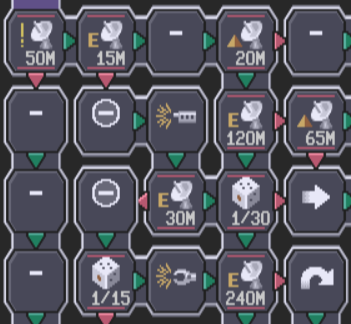
\includegraphics[width=0.5\textwidth]{img/CarnageHeartSoftware.png}
  \caption{Screenshot of the programming interface in Carnage Heart.\cite{carnageheartsoftware}}
  \label{fig:carnageheartsoftware}
\end{figure}

'Carnage Heart' teaches basic programming constructs, but it does not present them as such. Instead the player is presented with a set of rules, which are much like the rules of programming, and are told to create what is basically an AI for the robot.\newline

Another example of a game trying to teach programming is 'CodeCombat'. \cite{codecombat} 'CodeCombat' is a browser-based game, that tries to teach JavaScript programming by making the player write code to play an RPG. The player plays as a wizard, and the programming is represented as magic spells in the game. The player is programming an AI for a knight, that has to fight a variety of monsters. Control of the knight includes movement and attack as well as conditions such as attack if the enemy is in range.
Although 'CodeCombat' is a game, it is very explicit in its teaching, because the player has to write the code and not just drag objects around on the screen. Tools such as 'Codecademy' provide the same kind of programming guides as 'CodeCombat', but without the gaming aspect.\cite{codecademy}\newline

Microsoft has released a game for teaching children programming called 'Kodu Game Lab'.\cite{kodu}
'Kodu Game Lab' is a free game on the PC and can be bought for $\$4.99$ on the Xbox360 marketplace.
This means, that the game is available to most possible users.\todo{To Martin: The game is available to both PC and XBOX users, so I do not feel that we can criticize it for being platform dependent.}
In the game, the player starts with a small world, which is a square of grass.
The player can then add objects and program them to do what the player wants.
It is possible to make an object react to other objects, e.g. eat them if the object is above the another object.
The programming interface for 'Kodu Game Lab' shown on \autoref{fig:kodu} is structured in a input/react way, that visually illustrates what will happen when some condition is met. This is is basic principal of if-statements, but the game does not include constructs such as loops or variable declaration, which will be a part of our final product. However, the simple drag-and-drop and click approach to programming avoids the need for the user to write code, thereby limiting how explicit the learning process is in the game.

\begin{figure}[ht]
  \centering
    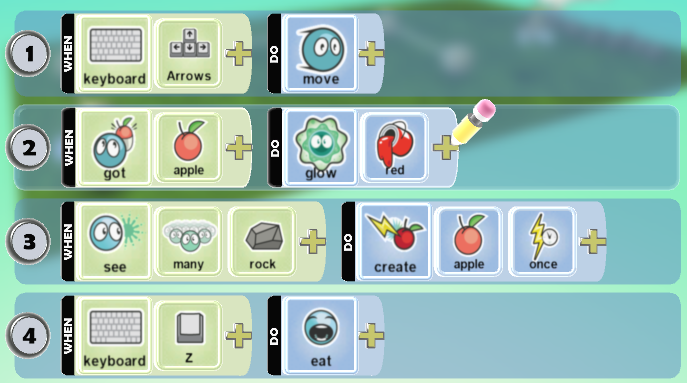
\includegraphics[width=\textwidth]{img/kodu.png}
  \caption{Screenshot of the programming interface in Kodu Game Lab.}
  \label{fig:kodu}
\end{figure}

The way 'Carnage Heart' and 'Kodu Game Lab' approach teaching basic programming constructs is relevant to our project, since they approach similar approaches to teaches basic programming constructs and could therefore be a source of inspiration in the design phase of this project.\todo{From Martin: If you will have time try to be more specific how these games are relevant for your project.}